\begin{figure}[!htb]
  \centering
  \begin{subfigure}{0.08\textwidth}
    \centering
    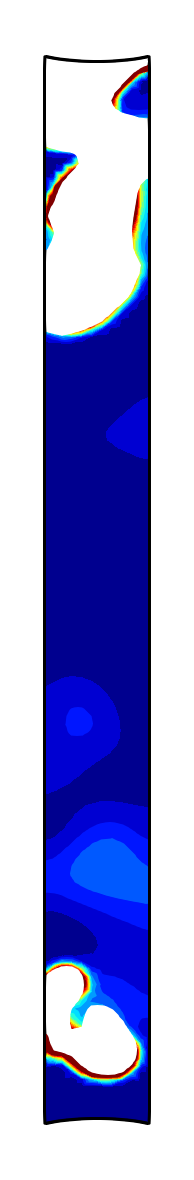
\includegraphics[width=\textwidth]{Chapter5/figures/spallation/psii_1}
  \end{subfigure}
  \begin{subfigure}{0.08\textwidth}
    \centering
    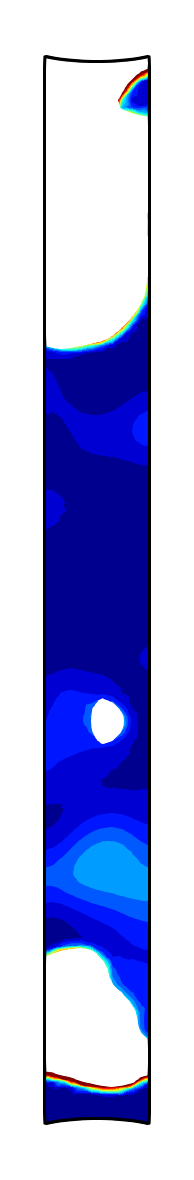
\includegraphics[width=\textwidth]{Chapter5/figures/spallation/psii_2}
  \end{subfigure}
  \begin{subfigure}{0.08\textwidth}
    \centering
    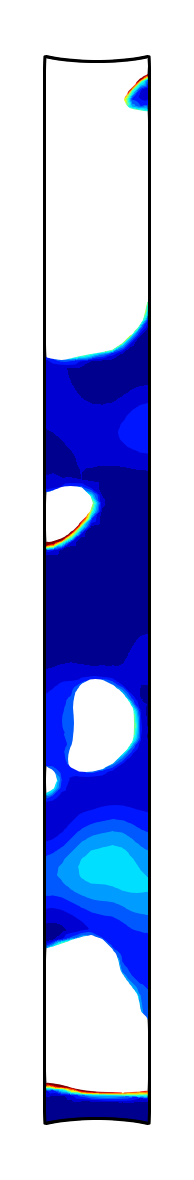
\includegraphics[width=\textwidth]{Chapter5/figures/spallation/psii_3}
  \end{subfigure}
  \begin{subfigure}{0.08\textwidth}
    \centering
    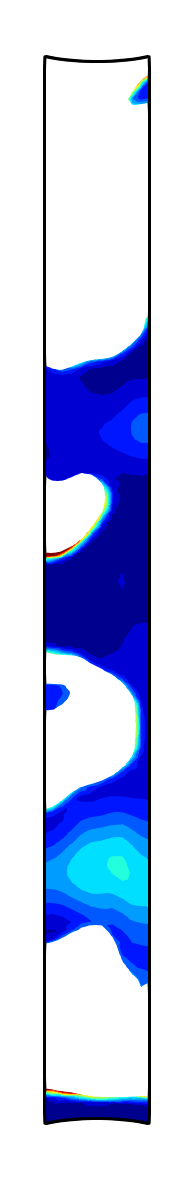
\includegraphics[width=\textwidth]{Chapter5/figures/spallation/psii_4}
  \end{subfigure}
  \begin{subfigure}{0.08\textwidth}
    \centering
    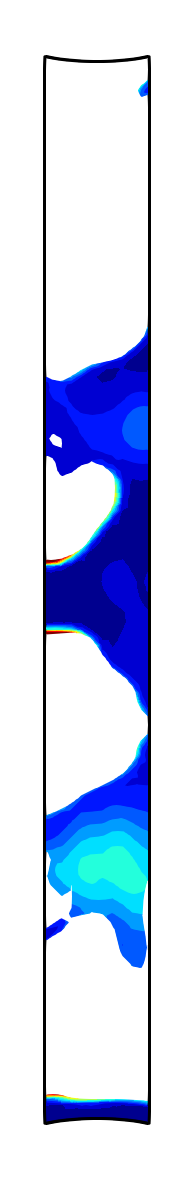
\includegraphics[width=\textwidth]{Chapter5/figures/spallation/psii_5}
  \end{subfigure}
  \begin{subfigure}{0.08\textwidth}
    \centering
    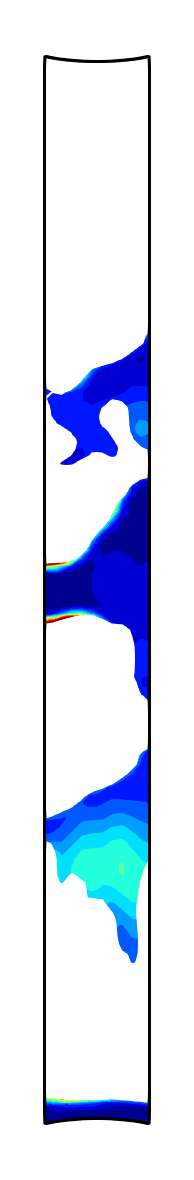
\includegraphics[width=\textwidth]{Chapter5/figures/spallation/psii_6}
  \end{subfigure}
  \begin{subfigure}{0.08\textwidth}
    \centering
    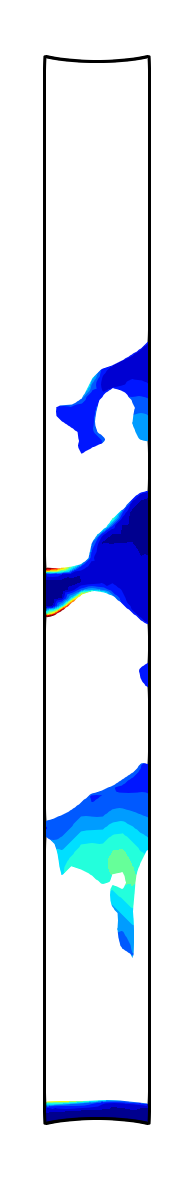
\includegraphics[width=\textwidth]{Chapter5/figures/spallation/psii_7}
  \end{subfigure}
  \begin{subfigure}{0.08\textwidth}
    \centering
    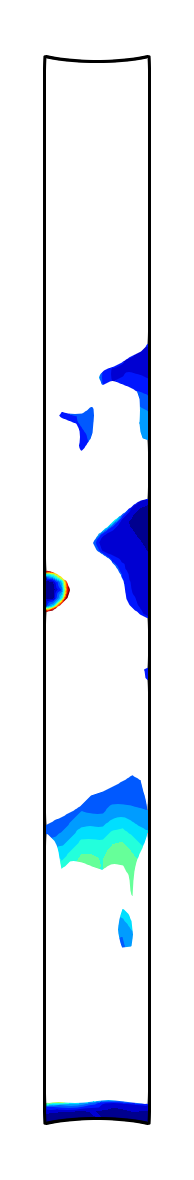
\includegraphics[width=\textwidth]{Chapter5/figures/spallation/psii_8}
  \end{subfigure}
  \begin{subfigure}{0.08\textwidth}
    \centering
    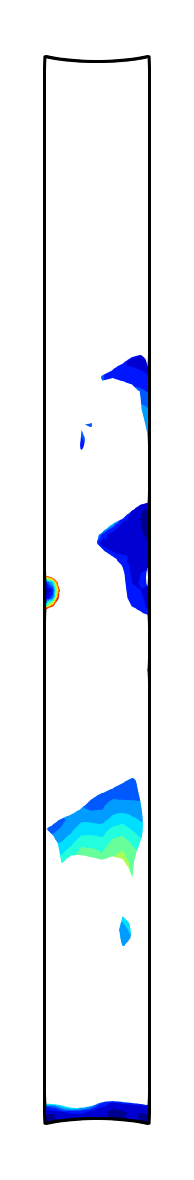
\includegraphics[width=\textwidth]{Chapter5/figures/spallation/psii_9}
  \end{subfigure}
  \begin{subfigure}{0.08\textwidth}
    \centering
    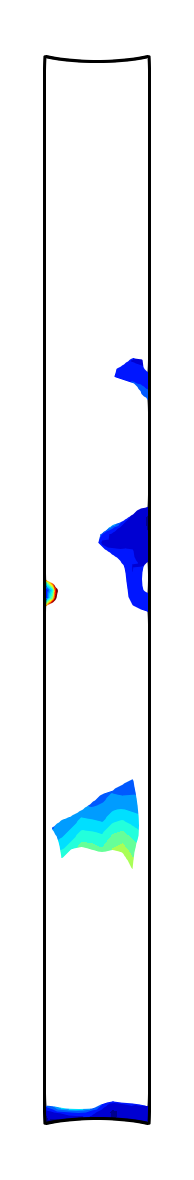
\includegraphics[width=\textwidth]{Chapter5/figures/spallation/psii_10}
  \end{subfigure}
  \begin{subfigure}{0.1\textwidth}
    \centering
    \caption*{$\psi^i_\activepart$}
    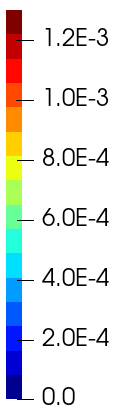
\includegraphics[width=\textwidth]{Chapter5/figures/spallation/colorbar_psii}
  \end{subfigure}
  \caption[The active interface energy density right after each shut-down event.]{The active interface energy density right after each shut-down event. The region within the contour of $c \leqslant 0.75$ is removed to visualize out-of-plane debonding.}
  \label{fig: Chapter5/spallation/animation_psii}
\end{figure}
